\documentclass[11pt]{article}
\usepackage{amsmath, amssymb, amsfonts,  graphicx, enumerate, float, wrapfig, hyperref}
\usepackage[margin=0.5in]{geometry}
\graphicspath{{./}}
\newcommand*{\vs}{\vspace{1cm}}
\newcommand*{\next}{\noindent}
\newcommand*{\set}{\setcounter{equation}{0}}

\begin{document}

\title{3.7 Optimization Problems}
\author{Juan J. Moreno Santos}
\date{November 2023}

\maketitle
\section{Numerical, Graphical and Analytic Analysis}
2. An open box of maximum volume is to be made from a square piece of material, 24 inches on a side, by cutting equal squares from the cornes and turning up the sides (see figure).\\
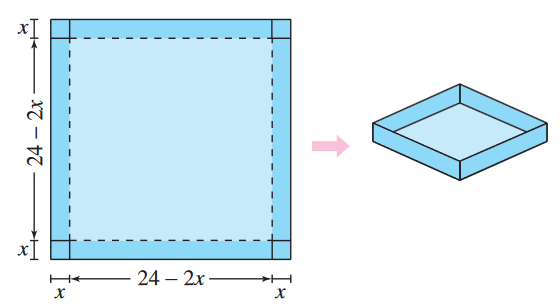
\includegraphics{2.png}\\
\begin{enumerate}[(a)]
    \item Analytically complete six rows of a table such as the one below. (The first two rows are shown.) Use the table to guess the maximum volume.
        \begin{flushleft}
            \begin{table}[h]
                \begin{tabular}{|l|l|l|}
                \hline
                Height $x$ & Length and Width & Volume $V$\\\hline
                $1$ & $24-2(1)$ & $1(24-2(1))^2=484$\\\hline
                $2$ & $24-2(2)$ & $2(24-2(2))^2=800$\\\hline
                $3$ & $24-2(3)$ & $3(24-2(3))^2=972$\\\hline
                $4$ & $24-2(4)$ & $4(24-2(4))^2=1024$\\\hline
                $5$ & $24-2(5)$ & $5(24-2(5))^2=980$\\\hline
                $6$ & $24-2(6)$ & $6(24-2(6))^2=864$\\\hline
                \end{tabular}
            \end{table}
        \end{flushleft}
        The maximum volume is given at $x=4$
    \item Write the volume $V$ as a function of x.\\
        \[V=x(24-2x)^2,\,\, 0<x<12\]
    \item Use calculus to find the critical number of the function in part (b) and find the maximum value.
        \begin{align}
            \set
            \frac{dV}{dx}&=2x(24-2x)(-2)+(24-2x)^2\\
            &=(24-2x)(24-6x)\\
            &=12(12-x)(4-x)=0\,\,\text{when}\,\, x=12,\,\, 4
        \end{align}
        12 is not in the domain.
        \begin{align}
            \frac{d^2V}{dx^2}=12(2x-16)\therefore\frac{d^2V}{dx^2}<0\,\,\text{when}\,\, x=4
        \end{align}
        When $x=4$. $V=1024$ is the maximum volume.
    \item Use a graphing utility to graph the function in part(b) and verify the maximum volume from the graph.\\
        The maximum volume is 1024.
\end{enumerate}

\section{Find two positive numbers that satisfy the given requirements.}
4. The product is 185 and the sum is a minimum.
\begin{align}
    \set
    S=x+y=x+\frac{185}{x}\\
    \frac{dS}{dx}=1-\frac{185}{x^2}=0\,\,\text{when}\,\, x=\sqrt[]{185}\\
    \frac{d^2S}{dx^2}=\frac{370}{x^3}>0\,\,\text{when}\,\, x=185
\end{align}
The two numbers are $\,\,\sqrt[]{185}$.

\vs\next
8. The sum of the first number squared and the second number is 54 and the product is a maximum.
\begin{align}
    \set
    x^2+y&=54\\
    S=xy&=x(54-x^2)=54x-x^3\\
    \frac{dS}{dx}&=54x-3x^2=0\,\,\text{when}\,\, x=3\sqrt[]{2}\\
    \frac{d^2P}{dx^2}&=-6x<0\,\,\text{when}\,\, x=3\sqrt[]{2}
\end{align}
The two numbers are $x=3\sqrt[]{2}$ and $y=36$.

\section{Find the length and width of a rectangle that has the given perimeter and a maximum area.}
10. Perimeter: $P$ units
\begin{align}
    \set
    2x+2y&=P\\
    y&=\frac{P-2x}{2}=\frac{P}{2}-x\\
    A&+xy=x\left(\frac{P}{2}-x\right)=\frac{P}{2}x-x^2\\
    \frac{dA}{dx}&=\frac{P}{2}-2x=0\,\,\text{when}\,\,x=\frac{P}{4}\\
    \frac{d^2A}{dx^2}&=-2<0\,\,\text{when}\,\, x=\frac{P}{4}
\end{align}
$A$ is maximum when $x=y=\frac{P}{4}$ units. Therefore, this rectangle is a square.

\section{Find the length and width of a rectangle that has the given perimeter and a minimum perimeter.}
12. Area: $A$ square centimeters
\begin{align}
    \set
    xy&=A\\
    y&=\frac{A}{x}\\
    P&=2x+2y=2x+2\left(\frac{A}{x}\right)=2x+\frac{2A}{x}\\
    \frac{dP}{dx}&=2-\frac{2A}{x^2}=0\,\,\text{when}\,\, x=\sqrt[]{A}\\
    \frac{d^2P}{dx}&=\frac{4A}{x^3}>0\,\,\text{when}\,\, x=\sqrt[]{A}
\end{align}
P is minimum when $x=y=\sqrt[]{A}$cm. Therefore, this rectangle is a square.

\section{Find the point on the graph of the function that is closest to the given point.}
14.\begin{align}
    \set
    f(x)&=(x-1)^2,\,\,(-5, 3)\\
    d&=\sqrt[]{(x=5^2)+((x-1)^2-3)^2}\\
    &=\sqrt[]{(x^2+10x+25)+(x^4-4x^3+8x+4)}\\
    &=\sqrt[]{x^4-4x^3+x^2+18x+29}
\end{align}
$d$ is the smallest when the expression inside this radical is the smallest. Now, we need to find the critical numbers of
\begin{align}
    \set
    g(x)&=x^4-4x^3+x^2+18x+29\\
    g'(x)&=4x^3-12x^2+2x+18\\
    &=2(x+1)(2x^2-8x+9)=0\\
    x&=-1
\end{align}
Since $x=-1$ yields a minimum, (-1, 4) is the closest point to (-5, 3).

\section{Area}
18. A rectangular page is to contain 36 square inches of print. The margins of each side are $1\frac{1}{2}$ inches. Find the dimensions of the page such that the least amount of paper is used.
\begin{align}
    \set
    xy&=36\Rightarrow y=\frac{36}{x}\\
    A&=(x+3)(y+3)=(x+3)\left(\frac{36}{x}+3\right)\\
    &=36+\frac{108}{x}+3x+9\\
    \frac{dA}{dx}&=-\frac{108}{x^2}+3=0\Rightarrow 3x^2=108\Rightarrow x=6,\,\, y=6
\end{align}
Therefore, the dimensions of the page are 9x9 inches.

\section{Traffic control}
20. On a given day, the flow rate $F$ (cars per hour) on a congested roadway is \[F=\frac{v}{22+0.02v^2}\]\\
where $v$ is the speed of the traffic in miles per hour. What speed will maximize the flow rate on the road?
\begin{align}
    \set
    \frac{dF}{dV}&=\frac{22-0.02v^2}{(22+0.02v^2)^2}\\
    &=0\,\,\text{when}\,\, v=\sqrt[]{1100}\approx 33.17
\end{align}
The flow rate on the road is maximized when the speed of traffic is 33mi/h.

\section{Maximum Area}
22. A rancher has 400 feet of fencing in which to enclose two adjacent rectangular corrals (see figure). What dimensions should be used so that the enclosed are will be a maximum?\\
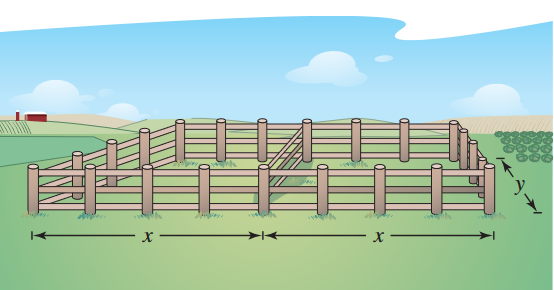
\includegraphics{22.png}\\
\begin{align}
    \set
    400ft&=4x+3y\\
    x&=\frac{400-3y}{4}\\
    Area=A&=2x\cdot y\\
    &=2\left(\frac{400-3y}{4}\right)y\\
    &=200y-\frac{3}{2}y^2\\
    A'&=200-3y=0
    y=\frac{200}{3}
\end{align}
Solving for x:
\begin{align}
    400&=3\left(\frac{200}{3}\right)+4x\\
    200&=4x\\
    50&=x
\end{align}
Since the fence is $2x$, the dimensions of the enclosed area will be 100ft by $\frac{200}{3}$ft.

\section{Maximum Volume}
24. Determine the dimensions of a rectangular solid (with a square base) with maximum volume if its surgace area is 377.5 square centimeters.
\begin{align}
    \set
    S&=2x^2+4xy=337.5\\
    y&=\frac{337.5-3x^2}{4x}\\
    V&=x^2y=x^2\left(\frac{337.5-2x^2}{4x}\right)=84.275-\frac{1}{2}x^3\\
    \frac{dV}{dx}&=84.375-\frac{3}{2}x^2=0\Rightarrow x^2=56.25\Rightarrow 56.25\Rightarrow x=7.5\,\,\text{and}\,\, y=7.5\\
    \frac{d^V}{dx^2}&=-3x<0\,\,\text{when}\,\, x=7.5
\end{align}
The maximum volume occurs when $x=y=7.5$cm.

\section{Maximum Area}
26. A rectangle is bounded by the $x-$ and $y-$axes and the graph of $y=\frac{6-x}{2}$ (see figure). What length and width should the rectangle have so that its area is a maximum?\\
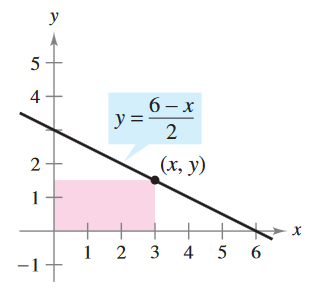
\includegraphics{26.png}\\
\begin{align}
    \set
    A&=xy\,\,\,\text{and}\,\,\, y=\frac{6-x}{2}\\
    A&=x\left(\frac{6-x}{2}\right)=\frac{1}{2}(6x-x^2)\\
    \frac{dA}{dx}&=\frac{1}{2}(6-2x)=0\,\,\text{when}\,\, x=3\\
    \frac{d^2A}{dx^2}&=-1<0\,\,\text{when}\,\, x=3
\end{align}
The rectangle should have a length and width of $x=3$ and $y=\frac{3}{2}$.

\section{Area}
30. Find the dimensions of the largest rectangle that can be inscribed in a semicircle of radius $r$.\\
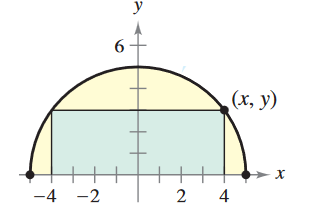
\includegraphics{30.png}
\begin{align}
    A&=2xy=2x\sqrt[]{r^2-x^2}\\
    \frac{dA}{dx}&=\frac{2(r^2-2x^2)}{\sqrt[]{r^2-x^2}}=0\,\,\text{when}\,\, x=\frac{\sqrt[]{2}r}{2}
\end{align}
The largest rectangle has dimensions $\sqrt[]{2}r$ by $\frac{\sqrt[]{2}r}{2}$.

\section{Numerical, Graphical, and Analytic Analysis}
A right circular cylinder is to be designed to hold 22 cubic inches of a soft drink (approximately 12 fluid ounces).
\begin{enumerate}[(a)]
    \item Analytically complete six rows of a table such as the one below (The first two rows are shown).
        \begin{flushleft}
            \begin{table}[h]
                \begin{tabular}{|l|l|l|}
                \hline
                    Radius $r$ & Height & Surface Area\\\hline
                    0.2 & $\frac{22}{\pi(0.2)^2}$ & $2\pi(0.2)\left(0.2+\frac{22}{\pi(0.2)^2}\right)\approx 220.3$\\\hline
                    0.4 & $\frac{22}{\pi(0.4)^2}$ & $2\pi(0.4)\left(0.4+\frac{22}{\pi(0.4)^2}\right)\approx 111$\\\hline
                    0.6 & $\frac{22}{\pi(0.6)^2}$ & $2\pi(0.6)\left(0.6+\frac{22}{\pi(0.6)^2}\right)\approx 75.6$\\\hline
                    0.8 & $\frac{22}{\pi(0.8)^2}$ & $2\pi(0.8)\left(0.8+\frac{22}{\pi(0.8)^2}\right)\approx 59$\\
                \hline
                \end{tabular}
            \end{table}
        \end{flushleft}
    \item Use a graphing utility to generate additional rows of the table. Use the table to estimate the minimum surface area.
    \begin{flushleft}
        \begin{table}[h]
            \begin{tabular}{|l|l|l|}\hline
                Radius $r$ & Height & Surface Area\\\hline
                0.2 & $\frac{22}{\pi(0.2)^2}$ & $2\pi(0.2)\left(0.2+\frac{22}{\pi(0.2)^2}\right)\approx 220.3$\\\hline
                0.4 & $\frac{22}{\pi(0.4)^2}$ & $2\pi(0.4)\left(0.4+\frac{22}{\pi(0.4)^2}\right)\approx 111$\\\hline
                0.6 & $\frac{22}{\pi(0.6)^2}$ & $2\pi(0.6)\left(0.6+\frac{22}{\pi(0.6)^2}\right)\approx 75.6$\\\hline
                0.8 & $\frac{22}{\pi(0.8)^2}$ & $2\pi(0.8)\left(0.8+\frac{22}{\pi(0.8)^2}\right)\approx 59$\\\hline
                1.0 & $\frac{22}{\pi(1.0)^2}$ & $2\pi(1.0)\left(1.0+\frac{22}{\pi(1.0)^2}\right)\approx 50.3$\\\hline
                1.2 & $\frac{22}{\pi(1.2)^2}$ & $2\pi(1.2)\left(1.2+\frac{22}{\pi(1.2)^2}\right)\approx 45.7$\\\hline
                1.4 & $\frac{22}{\pi(1.4)^2}$ & $2\pi(1.4)\left(1.4+\frac{22}{\pi(1.4)^2}\right)\approx 43.7$\\\hline
                1.6 & $\frac{22}{\pi(1.6)^2}$ & $2\pi(1.6)\left(1.6+\frac{22}{\pi(1.6)^2}\right)\approx 43.6$\\\hline
                1.8 & $\frac{22}{\pi(1.8)^2}$ & $2\pi(1.8)\left(1.8+\frac{22}{\pi(1.8)^2}\right)\approx 44.8$\\\hline
                2.0 & $\frac{22}{\pi(2.0)^2}$ & $2\pi(2.0)\left(2.0+\frac{22}{\pi(2.0)^2}\right)\approx 47.1$\\\hline
            \end{tabular}
        \end{table}
    \end{flushleft}
        The minimum is 43.6 for $r=1.6$ \newpage
    \item Write the surface area $S$ as a function of $r$.
        \begin{align}
            \set
            S&=2\pi r^2+2\pi rh\\
            &=2\pi r(r+h)\\
            &=2\pi r\left(r+\frac{22}{\pi r^2}\right)\\
            &=2\pi r^2+\frac{44}{r}
        \end{align}
        \item Use a graphing utility to graph the funciton in part (c) and estimate the minimum surface area from the graph.\\
            The minimum is about 4.5 for $r\approx 1.5$.
        \item Use calculus to find the critical number of the function in part (c) and find dimensions that will yield the minimum surface area.
            \begin{align}
                \set
                \frac{dS}{dr}&=4\pi r-\frac{44}{r^2}=0\,\,\text{when}\,\, r=\sqrt[3]{\frac{11}{\pi}}\approx 1.52\text{in}\\
                h&=\frac{22}{\pi r^2}\approx 3.04\text{in}
            \end{align}
\end{enumerate}

\section{Capstone}
38. The perimeter of a rectangle is 20 feet. Of all possible dimensions, the maximum area is 25 square feet when its length and width are both 5 feet. Are there dimensions that yield a minimum area? Explain.\\
\indent the isn't a minimum area. If we let the sides be $x$ and $y$ then
\begin{align}
    \set
    2x+2y=20\\
    y=10-x
\end{align}
The area would be 
\begin{align}
    A(x)&=x(10-x)\\
    &=10-x^2
\end{align}
This can be made indiscriminately small if x approaches 0.

\section{Minimum cost}
40. An industrial tank of the shape describe of the shape described in Exercise 30 ["two hemispheres adjoined to the ends of a right circular cilinder"] must have a volume of 4000 cubic feet. The hemispherical ends cost twice as mch per square foot of surface area as the sides Find the dimensions that will minimize cost.\\
\indent Let lowercase $c$ be the cost per surface area's ft$^2$.\\
$2c$ would be the hemispherical ends' cost per ft$^2$.
\begin{align}
    C&=2c(4\pi r^2)+c(2\pi rh)\\
    &=c(8\pi r^2+2\pi r\left(\frac{4000}{\pi r^2}-\frac{4}{3}r\right))\\
    &=c\left(\frac{16}{3}\pi r^2+\frac{8000}{r}\right)\\
    \frac{dC}{dr}&=c\left(\frac{32}{3}\pi r-\frac{8000}{r^2}\right)=0\,\,\text{when}\,\, r=\sqrt[3]{\frac{750}{\pi}}\\
    &\approx 6.204\text{ft}\,\,\text{and}\,\, h\approx 24.814\text{ft}
\end{align}
The dimensions that will minimize cost are $r=\sqrt[3]{\frac{750}{\pi}}$ and $h\approx 24.814$ft.

\section{Minimum cost}
54. An offshore oil well is 2 kilometers off the coast. The refinery is 4 kilometers down the coast. Laying pipe in the ocean is twice as expensive as on land. What path should the pipe follow in order to minimize the cost?
\begin{align}
    \set
    C(x)&=2c\sqrt[]{x^2+4}+c(4-x)\\
    C'(x)&=\frac{2xk}{\sqrt[]{x^2+4}}-k=0\\
    2x&=\sqrt[]{x^2+4}\\
    4x^2&=x^2+4\\
    3x^2&=4\\
    x&=\frac{2}{\sqrt[]{3}}
\end{align}

\section{Maximum Profit}
58. Assume that the amount of money deposited in a bank is proportional to the square of the interest rate the bank pays on this money. Furthermore, the bank can reinvest this money at 12\%. Find the interest rate the bank should pay to maximize profit (Use the simple interest formula.)\\
\indent Let $m$ be the money desposited, $p$ the profit, and $i$ the interest paid.
\begin{align}
    p&=(0.12)m-im\\
    m&=ki^2\\
    p&=(0.12)(ki^2)-i(ki^2)=k(0.12i^2-i^3)\\
    \frac{dp}{di}&=k(0.24i-3i^2)=0\,\,\text{when}\,\, i=\frac{0.24}{3}=0.08\\
    \frac{d^2p}{di^2}&=k(0.24-6i)<0\,\,\text{when}\,\, i=0.08
\end{align}
The profit is maximized when the interest rate is at 8\%.

\section{Diminishing returns}
The profit $P$ (in thousands of dollars) for a company spending an amount $s$ (in thousands of dollars) on advertising is
\[P=-\frac{1}{10}s^3+6s^2+400\]
\begin{enumerate}[(a)]
    \item Find the amount of money the company should spend on advertising in order to yield a maximum profit.
        \begin{align}
            \set
            \frac{dp}{ds}&=-\frac{3}{10}s^2+12s\\
            &=-\frac{3}{10}s^2(s-40)\\
            &=0\,\,\text{when}\,\, x=0\,\,\text{and}\,\, s=40\\
            \frac{d^2p}{ds^2}&=-\frac{3}{5}s+12\\
            \frac{d^2p}{ds^2}&(0)>0,\,\, s=0\,\,\text{gives a minimum.}\\
            \frac{d^2p}{ds^2}&(40)<0,\,\, s=40\,\,\text{gives a maximum.}
        \end{align}
        The company should spend \$40000 (from $s=40$) in order to yield a maximum profit of $p=\$3600000$.
    \item The point of diminishing returns is the point at which the rate of growth of the profit funciton begins to decline. Find the point of diminishing returns.
        \begin{align}
            \set
            \frac{d^2p}{ds^2}=-\frac{3}{5}s+12=0\,\,\text{when}\,\, s=20
        \end{align}
        The point of diminishing returns happens at $s=20$, which is \$20000 spent on advertising.
\end{enumerate}































\end{document}